%% [ADS 4-2005] Template file for 40in x 30in landscape poster
%%
%%
%%
%%
%% [ADS 4-2005] what follows here is obsolete I believe.
%%-------------------------------------------------------------------------
%% Written by Graeme, 2001-03 based on Norman's original microlensing
%% poster.
%%
%% $Id: poster-template-landscape.tex,v 1.1 2001/07/02 17:23:32 norman Exp $
%%
%% Default mode is landscape, which is what we want, however dvips and
%% a0poster do not quite do the right thing, so we end up with text in
%% landscape style (wide and short) down a portrait page (narrow and
%% long). Printing this onto the a0 printer chops the right hand edge.
%% However, 'psnup' can save the day, reorienting the text so that the
%% poster prints lengthways down an a0 portrait bounding box.
%%
%% 'psnup -w85cm -h119cm -f poster_from_dvips.ps poster_in_landscape.ps'
%%
%%-------------------------------------------------------------------------
%% Modified by Ronald Kumon, 06-2002 to incorporate a framebox border,
%%   add acknowledgments line at bottom, and change locations of logos
%%
%% Modified by Anand D. Sarwate 04-2005 to specialize to the UC Berkeley 
%%   EECS Wireless Foundaions conference poster template and for different
%%   paper sizes


%% [ADS 4-2005] latex --> dvips --> ps2pdf works just fine for me.
%%
%% To preview using xdvi:
%% 
%% $ xdvi -paper 1188x840mm -s 24 -nopostscript poster.dvi
%%
%% To convert dvi to Postscript:
%%
%% $ dvips -Ppdf -G0 -o poster.ps poster.dvi
%%
%% The dvips options are:
%% Ppdf: use the PDF printer configuration file
%% G0  : shift lower characters to higher position 
%%       (splits ligatures when using Times-Roman font)
%%
%% To convert Postscript to PDF:
%%
%% $ pstill -c -giptCQ -w 3368 -h 2378 -o poster.pdf poster.ps
%% ($ pstill -c -iptCQ -w 3225 -h 2378 -o poster.pdf poster.ps)
%%
%% Note that the pstill options are
%% c:  compression (more c's give more compression; up to four)
%% g:  take size from Postscript file
%% p:  include all fonts as partial fonts
%% i:  include all non-standard fonts
%% t:  map graphics transfer functions from PostScript to PDF. 
%% C:  use RGB color map
%% w:  width in points (1/72 inch) for 1188 mm
%% h:  height in points (1/72 inch) for 839 mm
%% Q:  take embedded fonts from PSFonts directory, not Postscript file
%% Note also that the -w and -h options need to be included else
%% some of the Postscript figures may not be displayed (particularly
%% those converted using fig2dev), even if the -g option is specified.
%% Also, the newest version of pstill (1.55.91) does not deal well with 
%% slanted Times Roman font; use italics or the older version (1.55.3). 
%%-------------------------------------------------------------------------


\documentclass{article}
%% [ADS 4/2005]  The template here does NOT make use of the 'slides'
%% option of Kumon in the interest of creating a more readable document
%% -- suggestions for how to make a backup style on separate sheet is
%% given in the text.
%%

%% If you want to number equations, set the equation number counter to zero.
%\setcounter{secnumdepth}{0}









%%%%%%%%%%%%%%%%%%%%%%%%%
%%% PACKAGE INCLUSION %%%
%%%%%%%%%%%%%%%%%%%%%%%%%

%% AMS packages for special symbols, etc
\usepackage{amsmath,amssymb}

%% This package gives you coloured text and various other simple
%% graphics hacks.  For details, see documentation in 
%% in /usr/local/teTeX/texmf/doc/generic/pstricks/*
\usepackage{pstricks}
\newrgbcolor{darkblue}{0.1 0.1 0.5}

%% The textpos package is necessary to position textblocks at arbitary 
%% places on the page.  Use showboxes option to show outlines of textboxes.
\usepackage[absolute]{textpos}
%\usepackage[absolute,showboxes]{textpos}

%% Package to include graphics.  
\usepackage{graphicx}
%% Define path for figures -- for safety, keep the last /
\graphicspath{{/your/figure/directory/here/if/any/}
{/an/second/directory/path/can/go/here/}}

%% Wrap text around figures
%\usepackage{wrapfig}

%% Use Times font instead of Computer Modern -- this gives better
%% appearance when resizing to large sixes.
%% Note that without the ``G0'' in the dvips conversion, 
%% all character combinations that will normally result in 
%% ligatures will have to be hacked to display properly.  For example, 
%%     fi --> \mbox{f}\mbox{i}
%% Other characters may also fail.  In addition, the Mathtimes font 
%% set should really be used for mathematics, but unfortunately they 
%% are only proprietary.  (The Computer Modern fonts may still look OK.)
\usepackage{times}

%% These colors are tried and tested for titles and headers. Don't
%% over use color!
%\usepackage[usenames]{color} % commented by Karol Kozio?
\usepackage{xcolor}
\definecolor{DarkBlue}{rgb}{0.1,0.1,0.5}
\definecolor{Black}{rgb}{0.0,0.0,0.0}
\definecolor{Red}{rgb}{0.9,0.0,0.1}
\definecolor{DarkBlue2}{rgb}{0.00,0.08,0.6}
\definecolor{DarkRed2}{rgb}{0.6,0.00,0.08}
\definecolor{DarkGreen2}{rgb}{0.00,0.6,0.08}
\definecolor{brilliantrose}{rgb}{1.0, 0.33, 0.64}
	\definecolor{darkpastelgreen}{rgb}{0.01, 0.75, 0.24}

%% Load shadow box package
%\usepackage{shadow}

%% This loads font sizes in style file a0size
\usepackage{a0size}





%%%%%%%%%%%%%%%%%%%%%%%%%%%%%%%% 
%%% NEW COMMAND DEFINTITIONS %%%
%%%%%%%%%%%%%%%%%%%%%%%%%%%%%%%%

%% See documentation for a0poster class for the size options here
%%    \normalsize will produce smaller type that might look too small
%%    \large will produce larger type
%% Feel free to modify if you want a different look
\let\Textsize\normalsize
%\let\Textsize\large
\def\RHead#1{\noindent\hbox to \hsize{\hfil{\LARGE\color{DarkBlue} #1}}\bigskip}
\def\LHead#1{\noindent{\LARGE\color{DarkBlue} #1}\bigskip}
\def\CHead#1{\begin{center}\noindent{\LARGE\color{DarkBlue} #1}\end{center}}
\def\Subhead#1{\noindent{\large\color{DarkBlue} #1}\bigskip}
\def\Title#1{\noindent{\textbf{\veryHuge\color{brilliantrose} #1}}}

\def\jHead#1{\begin{left}\noindent{\large\color{DarkBlue} #1}\end{left}}




%%%%%%%%%%%%%%%%%%%%%%%%%%%%%
%%% GLOBAL LAYOUT OPTIONS %%%
%%%   NUMBER OF COLUMNS   %%%
%%%%%%%%%%%%%%%%%%%%%%%%%%%%%

%% Set paper size
%% Depending on the conference, the posterboard size may be different.
%% This template was based on an ISO standard A0, which is in use everywhere
%% except for the United States.  A0 paper is  46.81 in x 33.11 in.
%% Depending on the posterboard size and the printer, you may need to 
%% change the widths and margins here.  Text width and height are set
%% in terms of paper width and height -- you can change margins here.
\setlength{\paperwidth}{40in}
\setlength{\paperheight}{30in}
\setlength{\textwidth}{36in}    %% paperwidth - (3in)
\setlength{\textheight}{26in}   %% paperheight - (3in)
\special{papersize=\the\paperwidth,\the\paperheight}
\typeout{Paper width and height are \the\paperwidth and \the\paperheight}
\typeout{Text width and height are \the\textwidth and \the\textheight}
%% Margins
\setlength{\headheight}{0cm}
\setlength{\headsep}{0cm}
\setlength{\topmargin}{1in}
\setlength{\topskip}{0cm}
\setlength{\oddsidemargin}{1in}
\setlength{\evensidemargin}{0in}
%% Font sizes
\renewcommand{\tiny}{\fontsize{12}{14}\selectfont}
\renewcommand{\scriptsize}{\fontsize{14.4}{18}\selectfont}   
\renewcommand{\footnotesize}{\fontsize{17.28}{22}\selectfont}
\renewcommand{\small}{\fontsize{20.74}{25}\selectfont}
\renewcommand{\normalsize}{\fontsize{24.88}{30}\selectfont}
\renewcommand{\large}{\fontsize{29.86}{37}\selectfont}
\renewcommand{\Large}{\fontsize{35.83}{45}\selectfont}
\renewcommand{\LARGE}{\fontsize{43}{54}\selectfont}
\renewcommand{\huge}{\fontsize{51.6}{64}\selectfont}
\renewcommand{\Huge}{\fontsize{61.92}{77}\selectfont}
\newcommand{\veryHuge}{\fontsize{74.3}{93}\selectfont}
\newcommand{\VeryHuge}{\fontsize{89.16}{112}\selectfont}
\newcommand{\VERYHuge}{\fontsize{107}{134}\selectfont}
%% skip lengths
\setlength{\smallskipamount}{6pt plus 2pt minus 2pt}
\setlength{\medskipamount}{12pt plus 4pt minus 4pt}
\setlength{\bigskipamount}{24pt plus 8pt minus 8pt}
\setlength{\abovecaptionskip}{25pt}
\setlength{\belowcaptionskip}{0pt}
\setlength{\abovedisplayskip}{25pt plus 6pt minus 15 pt}
\setlength{\abovedisplayshortskip}{0pt plus 6pt}
\setlength{\belowdisplayshortskip}{13pt plus 7pt minus 6pt}
\setlength{\belowdisplayskip}{\abovedisplayskip}

%% Set up the grid
%%
%% Note that [40mm,40mm] is the margin round the edge of the page
%% it is _not_ the grid size. That is always defined as 
%% PAGE_WIDTH/HGRID and PAGE_HEIGHT/VGRID. In this case we use
%% 46 x 26. This gives us 4 columns of width 10 boxes, with a gap of
%% width 2 in between them.  There are 26 vertical boxes.
%%
%% (Note however that texblocks can be positioned fractionally as well,
%% so really any convenient grid size can be used.)
%%
\TPGrid[40mm,40mm]{46}{26} % 4 cols of width 10, plus 3 gaps width 2

%% Text layout parameters
\parindent=0pt
\parskip=0.5\baselineskip





%%%%%%%%%%%%%%%%%%%%%
%%% THEOREMS, ETC %%%
%%%%%%%%%%%%%%%%%%%%%
\newtheorem{thm}{Theorem}






%%%%%%%%%%%%%%%%%%%%%%%%%%%%
%%% DOCUMENT BEGINS HERE %%%
%%%%%%%%%%%%%%%%%%%%%%%%%%%%

%% The basic format of the poster is to create text boxes with the
%% various things you want to display.  You can then play around 
%% with how to lay thing out.  In the old version of this template,
%% the content was always provided with alternatives suitable for
%% printing on sheets of paper (resizing fonts, images, etc).  I
%% think that's too confusing to read.  The old layout was:
%%     \ifposter
%%          some poster commands go here
%%     \else
%%          an alternative style here in case you are printing on
%%          regular sheets of paper
%%     \fi
%% One option is to make the entire poster and then wrap it in an \ifposter
%% and then make all the slides separately.  This seems to be easier
%% if your poster is not much like a bunch of 8.5x11 sheet tacked together
%% in the first place.
\begin{document}

%% Do not put page numbers at the bottom of the page for poster
\pagestyle{empty}



%% Declare proper hyphenation
\hyphenation{equi-bi-ax-i-al}
\hyphenation{in-fin-i-tes-i-mal}


%% Border and background options -- you can make up others if you
%% like.  These all use the pstricks package.
%% DRAW A BLUE BORDER AROUND THE POSTER USING PSTRICKS
\psset{linewidth=0.5cm}
% Sets up lengths for frame
\newlength{\frameleft}
\newlength{\frameright}
\newlength{\frametop}
\newlength{\framebottom}
\setlength{\frameleft}{-1in}
\setlength{\frameright}{\textwidth}
\addtolength{\frameright}{1in}
\setlength{\frametop}{1in}
\setlength{\framebottom}{-\textheight}
\addtolength{\framebottom}{-1in}
% Draws a blue frame
% \psframe[linecolor=darkblue,cornersize=absolute,linearc=2]
% (\frameleft,\framebottom)(\frameright,\frametop)% need to %  
%  %  overlay EOSMLS
% \psline{->}(0cm,0cm)(\textwidth,-\textheight)
%   *** End code to draw border *** 

%% USE A COLORED BACKGROUND FOR THE ENTIRE POSTER
%% [ADS 4-2005] THIS OPTION IS NOT SUPPORTED YET
%\newrgbcolor{gradbegin}{0.3 0.5 0.7}
%\newrgbcolor{LightBlue}{0.7 0.7 1.0}
%\psframe[fillstyle=solid,fillcolor=LightBlue](\frameleft,\framebottom)(\frameright,\frametop)



%% Adjust spacing in long displayed mathematical formulas to tighten them up
\setlength{\abovedisplayskip}{0.75\abovedisplayskip}
\setlength{\belowdisplayskip}{0.75\belowdisplayskip}



%% Understanding textblocks is the key to being able to do a poster in
%% LaTeX. The first argument gives the block width in grid cells, the
%% second gives the positioning on the grid.
%%
%% NOTE:  You will have to do a lot of previewing to get everything
%% in the right place.
%%
\begin{textblock}{46}(00,00)
\begin{center}
\Title{DGX Station A100  : For  Bigger Models, Faster Answers  }
\end{center}
\end{textblock}

\begin{textblock}{46}(00,01.5)    
\begin{center}
\LHead{MBUZZ and NVIDIA }\\
\LHead{\textit{\textcolor{darkpastelgreen}{GITEX GLOBAL 2022, DUBAI} }}
\end{center}
\end{textblock}


%% UCB EECS logo on left, Wireless Foundations Logo on right
\begin{textblock}{2}(00.5,01)
\begin{center}
\includegraphics[height=9cm,width=13cm]{SPv1a.pdf}
\end{center}
\end{textblock}

\begin{textblock}{8}(38,01)
\begin{center}
%\includegraphics[height=5cm]{wifound.eps} % modified by Karol Kozio?
\includegraphics[height=9cm,width=13cm]{a100boxv1.pdf}
\end{center}
\end{textblock}


\begin{textblock}{42}(02,03)
\begin{center}
% \rule{1200pt}{7pt}
\textcolor{brilliantrose}{\rule{1200pt}{7pt}}
\end{center}
\end{textblock}



%% Begin 1st row
\begin{textblock}{10}(00,05.2)
\CHead{Did you deploy AI service? }            
Nvidia DGX Station A100 is providing  an opportunity to use the world’s only office-friendly system with four fully interconnected and MIG-capable Nvidia A100 GPUs, leveraging Nvidia® NVLink® for running parallel jobs and multiple users without impacting system performance. Training platform is different from deployment platform. Same provides obstruction to deploy trained AI Model ( CNN, RNN networks , etc)  into limited capability deployment edge. Mostly there is a need to cut down AI Model size or optimise weights of AI Model. Optimization of AI Model size or  changing  weight AI Model may not be there if deployment happens  in edge side by using DGX Station A100.

\end{textblock}



\begin{textblock}{10}(00,11.2)
\CHead{Data Center on your Table}
DGX Station A100 is a server-grade AI system that doesn’t require data center power and cooling. It includes four NVIDIA A100 Tensor Core GPUs, a top-of-the-line, server-grade CPU, super-fast NVMe storage, and leading-edge PCIe Gen4 buses, along with remote management so you can manage it like a server. Suitable for use in a standard office environment without specialized power and cooling. 
\end{textblock}


\begin{textblock}{10}(00,15.2)
\CHead{DGX Station A100 at a Glance}
AI workgroup server delivering 2.5 peta FLOPS
Organizations around the world can provide multiple users with a centralized AI resource for all workloads that delivers an immediate on-ramp to Nvidia DGX™-based infrastructure and works alongside other Nvidia-Certified Systems with a DGX Station A100 rental now available from MBUZZ. With Multi-Instance GPU (MIG), it’s possible to allocate up to 28 separate GPU devices to individual users and jobs.

Including four Nvidia A100 Tensor Core GPUs, a top-of-the-line server-grade GPU, super-fast NVMe storage, and leading-edge PCIe Gen4 buses. A100 includes remote management so enterprise customer can manage their DGX  Station A100 like a server. With no complicated installation processes or significant IT infrastructure required, the DGX Station A100 can truly be placed anywhere enterprise customer data science team requires complex computations. Simply plug your Station into any standard wall outlet to get it up and running in minutes – and work from anywhere. 

This supercomputer was truly designed for today’s agile data science teams that work in corporate offices, labs, research facilities, or even from home – as the DGX Station A100 can run simultaneous processes from multiple users without affecting performance.
\end{textblock}



\begin{textblock}{10}(12,04)
\CHead{On-prem Requirement}
 Enterprise Business owners of all sizes are struggling to find the next generation AI solutions that will unlock the hidden patterns and value from their huge volume of data. Emerging AI enabled micro services in a given enterprise are driven by the confluence of ML/DL algorithms. Enterprise on-prem requirement appears to be matching with specifications of DGX Station A100 which is providing high levels of accuracy in Business Solutions. However, AI enabled enterprise service initiatives are complex and often require specialised skills, ability, hardware and software that is often not readily available. 
\end{textblock}




% \begin{textblock}{10}(12,31)
%  \CHead{How to include graphics}
%  hhhh
%  \end{textblock}




\begin{textblock}{10}(24,04)
\CHead{Engineering Resources}
MBUZZ is providing following services to Enterprise Business customers
\begin{itemize}
\item Training Data-Set creation (on-prem or in IBM cloud).
\item  Building AI model by using, Tensorflow or PyTorch.  Building AI model by using Custom framework \textcolor{brilliantrose}{DLtrain} ( for NN, limited version of CNN) 
\item  Training  AI model by using DGX Station A100
\item  Deploying  AI model  in IoT Edge for Inference service in real time.
\end{itemize}
\end{textblock}




\begin{textblock}{22}(12,9.1)
\CHead{Ready to use  in Enterprise Business for AI Workload}
\begin{center}
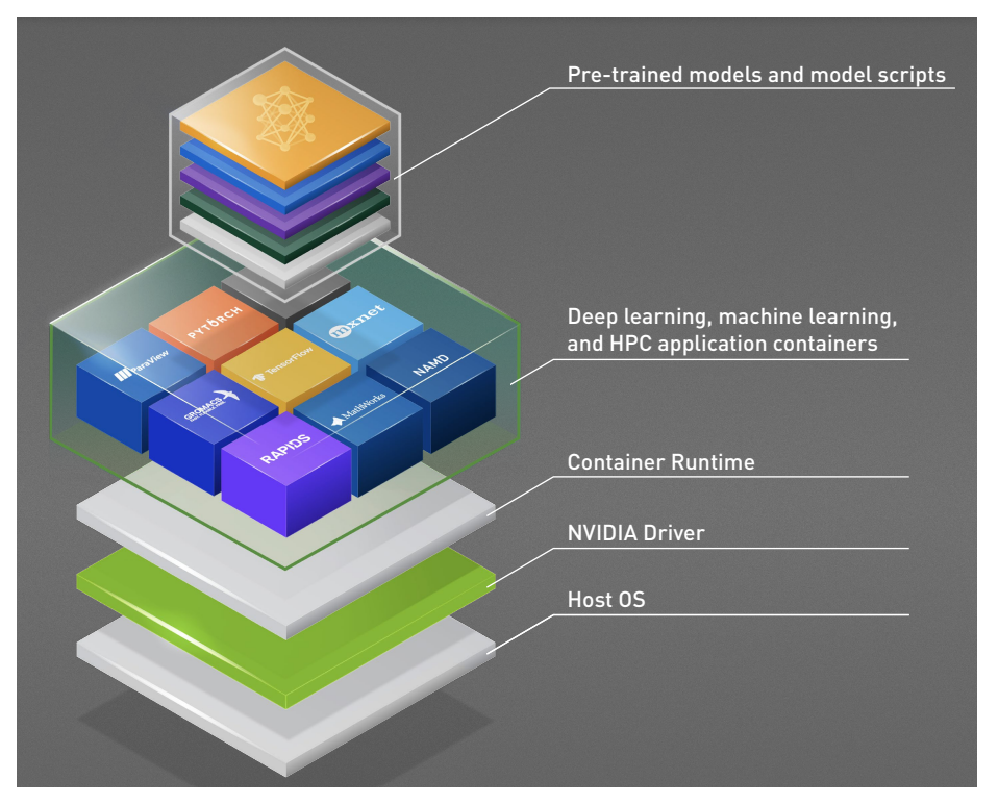
\includegraphics[width=18in]{a100v1a.eps}
\end{center}
\end{textblock}






\begin{textblock}{10}(36,05)
\CHead{Training, Inference, Analytics}
Enterprise customers have the option to  train large models using a fully GPU-optimized software stack and up to 320 gigabytes (GB) of GPU memory. With DGX Station A100, Enterprise  can provide multiple users with a centralized AI resource for all workloads—training, inference, data analytics.

DGX Station A100 brings AI out of the data centre with a server-class system that can plug in anywhere to perform real time Inference.

DGX Station A100  is using the NVIDIA DGX ™ software stack and  it is an ideal platform for teams from all Enterprises, large and small.

Data Science Teams Effortlessly providing multiple, simultaneous users with a centralised AI resource, DGX Station A100 is the work group appliance for the age of AI. It’s capable of running training, inference, and analytics workloads in parallel, and with MIG, it can provide up to 28 separate GPU devices to individual Data science teams.

\end{textblock}


\begin{textblock}{10}(36,14)
\CHead{Pre-trained models}
Get Results Sooner by using Pre-trained models, scripts, and more translate to better results sooner over do-it - yourself problem solving.Large-scale pre-trained models (PTMs) such as BERT and GPT. Recently, use of Pre-trained models have been   achieving great success and become an attractive milestone in the field of artificial intelligence (AI) for Enterprise Business owners. Owing to sophisticated pre-training objectives and huge model parameters, large-scale PTMs can effectively capture knowledge from massive labeled and unlabeled data.    By storing knowledge into huge parameters and fine-tuning on specific tasks, the rich knowledge implicitly encoded in huge parameters can benefit a variety of downstream tasks, which has been extensively demonstrated via experimental verification and empirical analysis. It is now the consensus of the AI community to adopt PTMs as backbone for downstream tasks rather than develop  learning models from scratch.

\end{textblock}


\begin{textblock}{10}(36,22)
\CHead{Custom framework for AI }
Custom AI framework is providing consistency across AI in IoT Edges. For example, Real time inference is  emerging as a critical need of the food and medical service delivery industry to   process and extract value from vast and diverse data sources that ensure high levels of  accuracy in delivered service. However, AI enabled enterprise service initiatives are complex and often require specialised skills, ability, hardware and software that is often not readily available. AI enabled application deployment requires deeply optimised and also production ready. 

\end{textblock}

\begin{textblock}{22}(12.3,24.4)
\jHead{\text{ Development  Platform : } }
Host OS is provided by NVIDIA and same is used by team in NVIDIA.   NVIDIA provides a Driver to handle A100 hardware from CPU. Most importantly "Container Runtime'' provides remote access to deploy containers for AI Model training. Enterprise Business  customers have the option to use their application containers for DL/ML.  Fresh AI model scripts or Pre-trained models can be used as an input to build AI applications.
 
\end{textblock}

% \begin{textblock}{30}(00,27.4)
% \begin{center}
\begin{textblock}{23}(12.3,26.4)
{\footnotesize Contact information:
U A E
Office #313
Al Nazr Plaza, Oud Metha
Dubai
Tel: +971 4 33 04 125
Fax: +971 4 33 04 099 \ \ -- 
Email: \textit{infor@mbuzz.com}; 
Web: \textit{https://www.mbuzztech.com/}
}
\vspace{-0.75\baselineskip}

{\footnotesize  hanks to all potential customers of DGX Station A100}
% \end{center}
\end{textblock}

\end{document}
